\chapter{ Cosmological simulations }


In cosmology one issue that currently exists is finding 
the dynamical evolution of the Universe, from its first 
stages to the actual epoch. This makes necessary tools to
study a big amount of interacting particles. 
Considering all possible components in the Universe evolution, 
the particles required to simulate the interaction among them
would be so huge that it would not be viable
to predict the evolution of every single particle for every
time step. 

In cosmological simulations a key component to consider
is dark matter, since it is mostly because of this one that 
the Universe has a filament structure. 
The latter asseveration is due to dark matter dominates the gravitational
interaction, not only because of its amount compared to
baryonic matter but also because it only interacts in this way.

This component cannot be observed directly cause it does not interact 
with radiation. But, since its gravitational effects are strong, there are 
observational evidence that accounts for its existence. For example, 
observing in galaxy rotation curves, the velocity measured at the outskirts 
was too fast to explain only with baryonic matter. 

A key argument to ignore baryonic matter in simulations is that
defining as total density the sum of baryonic and dark matter only, 
dark matter would contribute with around $80\%$ of all the density
content. 

The next chapter is divided in several sections, the first one
corresponds to the methods used in cosmological simulations to
calculate the gravitational evolution of the system. The second
one contains different criteria selection to detect a dark matter
halo in simulations. The third and fourth sections are dedicated
to explain how to build two different statistical measures of clustering
in real and fourier space, the correlation function and power spectrum 
respectively. 


%&&&&&&&&&&&&&&&&&&&&&&&&&&&&&&&&&&&&&&&&&&&&&&&&&&&&&&&&&&&&&&&&&&&&&&&&&&&&&&&&&&&&&&&&&&&&&&&&&&&&&&&&&&&&&&&&&&&&&&
\section{ Numerical methods }
%&&&&&&&&&&&&&&&&&&&&&&&&&&&&&&&&&&&&&&&&&&&&&&&&&&&&&&&&&&&&&&&&&&&&&&&&&&&&&&&&&&&&&&&&&&&&&&&&&&&&&&&&&&&&&&&&&&&&&&


In the last chapter the equations that describe the evolution of 
the perturbations in linear regime were provided and the Zeldovich 
approximation for non linear regime was also given. But in a cosmological
simulation is necessary initial conditions for the density field
or a initial shape of the power spectrum. In these cosmological simulations 
dark matter is a key component, in many cases is the only particle considered,
hence some observational evidences are going to be provided. As already stated
dark matter does not interact with radiation, the reason to be proposed 
is the gravitational effects found in different systems studied. It is 
about the  $\sim 24\%$ content of the Universe therefore it is important 
to study its evolution. 

One of the first observational evidence was found in the Coma cluster due to
a mass estimation from the virial theorem, let's see this in more detail  

the specific kinetic energy of the system is $T = v^2/2 \sim 3\sigma^2/2 $ 
where $\sigma$ is the galaxy velocity dispertion and the potential energy
is $U = 3GM_{vir}/(5R_{vir})$. From the mass-luminosity ratio and the 
mean luminosity of the cluster, a second estimative of the mass is found. There is
a discrepancy between the two values so big to assert that $\sim 90\%$ of the 
cluster's mass is not visible. 

The rotation curve of the galaxies can be other prove for dark matter existence,
for example, the velocity measures performed with respect to the radious of Andromeda 
galaxy (or another spiral galaxies) is approximately the same independent of the radial
distance of the stars to the center of the galaxy. From this it could be affirmed that
density is uniform along the galaxy contrary to expected for the observed 
number of star in function of the radious. 


The Bullet cluster is composed by two two clusters that are colliding, an event 
not commonly observed. The gas of them reaches velocities around $\sim 10$ $millions$ $of$ $miles/h$
during the violent collition while they interact among them because of their charge. 
This interaction disminishes the gas velocity but this does not happen with dark
matter cause it does not interact electrically. 
Using gravitational lensing a distortion map is obtained. Using the X rays detected
and the distortion map four different groups of matter are found, 2 bigger ones
that correspond to the dark matter component and two smaller ones that correspond
to luminous matter formed from the intercluster gas. These presents a strong
evidence of dark matter existence. 

\

Additionally to the initial conditions, the box size $L$ and the number of 
dark matter particles $N^3$ that would be used should be fixed. 
The gravitational interaction calculation of such a big number of particles
could in principle be calculated through direct calculation. This first
attempt is not very efficient or even it is not possible to perform it
since the computing time or the computational resources would be very 
big to be viable. The latter is the reason for approximate methods 
to appear as a possible solution that implies more reasonable computing times.

A main objective in a simulation could be the study the formation process, fusion and
further interactions that are produced among halos and vacuum regions that conform
the filamentary structure of the Universe. Next, three of the most known numerical 
methods for cosmological simulations are going to be briefly exposed.

\begin{enumerate}
\item \textbf{Particle Mesh (PM)}\cite{tree}

In this method a grid is created over the particle array
as shown in the figure \ref{PM}. The particles more closed
to a vertice are assigned to this, to an specific cell, getting the density. 
Other way to calculate the density is cloud in cell, later explained
in more detail, where particles are considered constant density cubes causing
that a single particle contributes to different cells.
Using Poisson equation the potential in every grid vertice can be found
thanks to the Fourier transform. The potential calculation or the force of 
each particle can be interpolated among the points created by the 
grid. 

Although this method reduces considerably the computing time 
since its of the order of O($N+M\log M$) with $N$ being the number of particles
and $M$ the number of vertices. The lack of resolution in the regions that are
more dense makes this method insufficient to respond for the physical situation.
Furthermore, it does not give account for a complex geometry or systems
higly correlated. A step forward in this direction is $P^3M$ that uses
for smaller scales finer calculations making a particle particle calculation. 

%**********************************************************************************************************************
\begin{figure}[htbp]
       \centering
               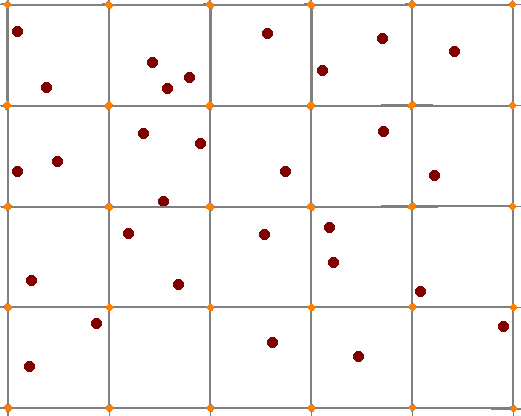
\includegraphics[width=0.35\textwidth]{Images/chapter3/MG.png}
       \caption{\small Particle mesh method. Every vertice of the grid gets 
       properties calculated from the closer particles.}
       \label{PM}
 \end{figure}
%**********************************************************************************************************************


\item \textbf{Tree method}\cite{tree}


To illustrate this method let's consider a 2D particle array. 
This square is divided in small cells of the same area where
each particle is assigned to a specific cell. 
If this number is superior to one, subdivisions of the cell
are performed and again if the number of particles per subcells 
is superior to one, subdivisions are made once more. This
process is repeated until for every cell there is at most
one particle. 
This subdivision is used to create a tree structure, this consists
in a root, i.e., all the square area and the branches that are 
created with each subdivision performed. This serves as a map
of the disposition of the particles in the square array. 
The particles are numerate from the upper left of the square 
until all particles in the first cell are numerate following with
the second cell until the lower left is reached. 

When the gravitational calculation is performed, the contribution 
to the force exerted over a particle due to the more distant ones
is much lower than with the nearer. Hence, the far ones can be 
approximated as a seudoparticle with mass $M$ and with a position
$r_{CM}=\sum_im_ir_i/M$. As a selection criteria the next expression
is taken

\begin{equation}
s/q\leq \theta
\label{sq}
\end{equation}

where $s$ is the cell size with wich the particle of interest is interacting 
with, $d$ the distance cell partilce and $\theta$ is a tolerance value to
define. When the condition is satisfied the gravitational interaction 
is calculated directly with the seudoparticle. In the opposite case the 
relation \ref{sq} for the subcells that contain the studied cell and that way
successively until the condition is satisfied or only one particle is 
present per cell. In this way the direct calculation is avoided for far
objects without avoiding the calculation for the nearer ones. 
Therefore, the computing time is reduced from $O(N^2)$ to $O(N\log(N))$.

%**********************************************************************************************************************
\begin{figure}[htbp]
       \centering
               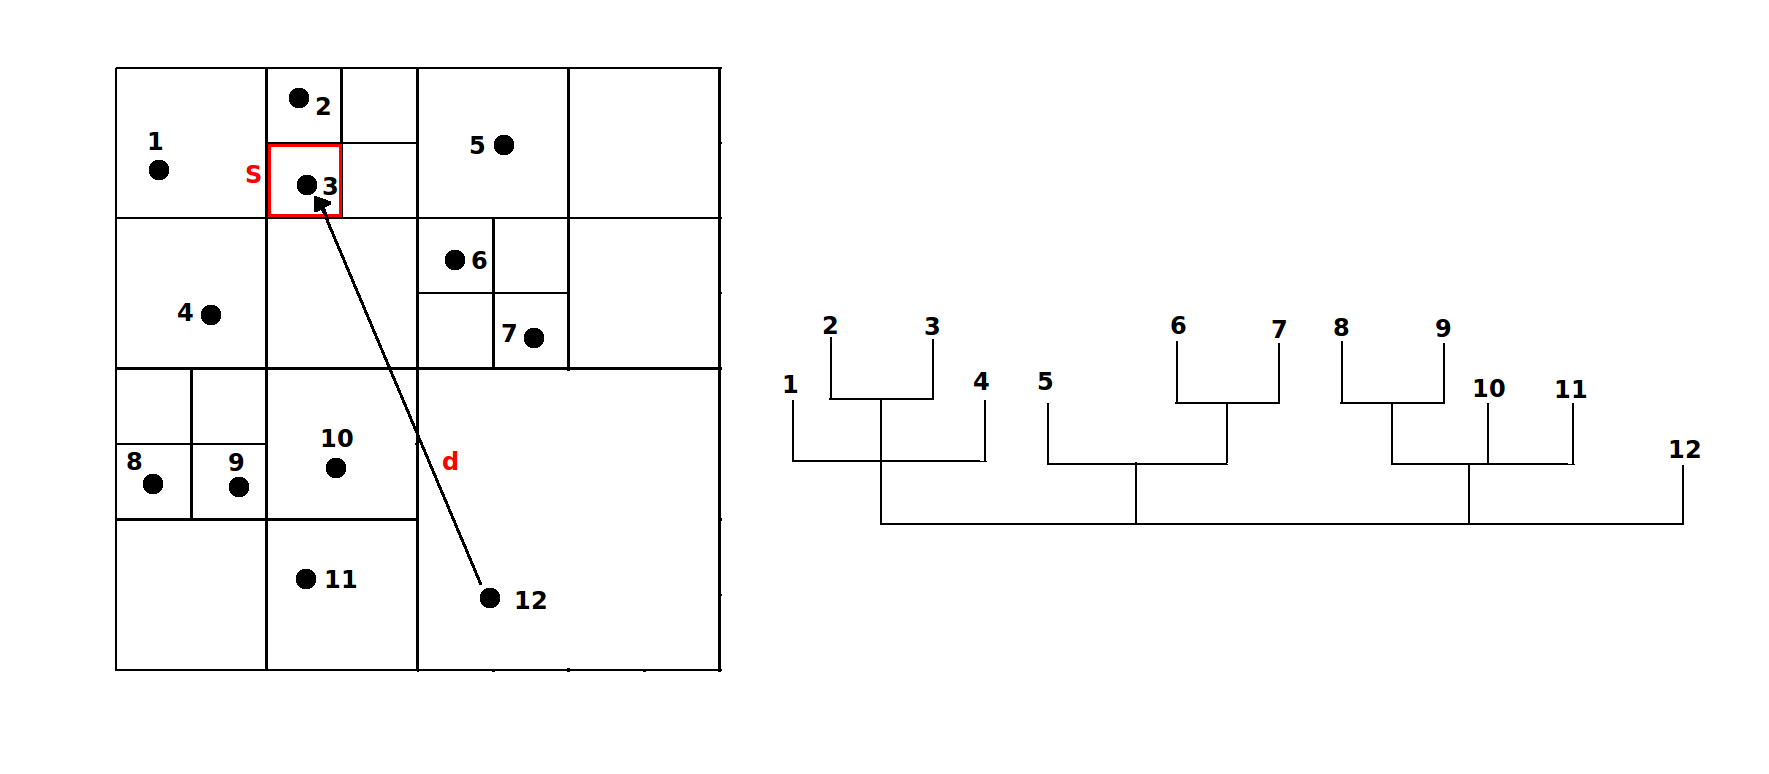
\includegraphics[width=1.0\textwidth]{Images/chapter3/treecode.png}
       \caption{\small In the left panel is shown the array of the particles and the subdivisions performed until at most one particle is found per cell. In the right one, the tree found for such distribution is shown.}
       \label{tree}
 \end{figure}
%**********************************************************************************************************************


\item ART Code\cite{klypin}

As its acronym indicates, Adaptive Refinement Tree Code consists in a multigrid
code. An initial grid is created where the Poisson equation is solved afterwards
followed by a refinement according to overdensities that are in certain regions.
Even after performing the refinement over the grid, this calculation can be 
continously being performed. Here, calculations particle particle are not being
performed. Something new compared to the methods previously exposed is that 
the cell shape can take any form allowing to get an adaptive grid depending on
the amount of particles in the region. 

\end{enumerate}

There are many methods that are hibrid among the 3 exposed, for example 
the already mentioned $P^3M$. All of them have both advantages and disadvantages
that need to be evaluated according to the needs of the simulation. 

\

%&&&&&&&&&&&&&&&&&&&&&&&&&&&&&&&&&&&&&&&&&&&&&&&&&&&&&&&&&&&&&&&&&&&&&&&&&&&&&&&&&&&&&&&&&&&&&&&&&&&&&&&&&&&&&&&&&&&&&&
\section{ Halo selection }
%&&&&&&&&&&&&&&&&&&&&&&&&&&&&&&&&&&&&&&&&&&&&&&&&&&&&&&&&&&&&&&&&&&&&&&&&&&&&&&&&&&&&&&&&&&&&&&&&&&&&&&&&&&&&&&&&&&&&&&

As a result of the dark matter particle interactions, perturbations 
grow enough to form ligated objects hence they are in virial equilibrium,
these are known as dark matter halos and satisfy $E_k=-V/2$. 
They are responsible for the potential wells that causes baryonic matter 
to fall in, finally forming the galaxies we observe today, i.e., dark
matter halos host galaxies. 

A main result of a cosmological simulation are the dark matter halos 
catalogue, which we are going to work with, that contains halo properties such
as position, velocity, mass, radious and redshift. Thus, a key step is to identify 
halos from a cosmological simulation, the methods generally use to acomplish such 
task are FOF and BDM 

\begin{enumerate}

%######################################################################################################################
\subsection{ Friends of friends }
%######################################################################################################################

\item Friend of Friends (FOF) 

To identify if a particles group lies in a dark matter halo, i.e., particles 
are linked, a length is defined such that all the particles that lie inside 
are part of the same group. This distance is called linking length. A condition 
is imposed, groups can not intersect among them, hence a particle can only belong 
to a specific group. But there is a problem with this approach, even when there is 
a little amount of particles in common between two groups, some sort of small 
``bridge`` that unites both of them, they are selected as one group not two
as would be expected. This method also allows to define substructures, therefore using
different linking lengths groups inside groups would be obtained, the bigger ones
would host the smaller ones. 

%######################################################################################################################
\subsection{ Bound density maximum }
%######################################################################################################################

\item Bound Density Maximun(BDM)

For this method the local maximum densities in the particle array of the simulation
are detected. From them a spherical cut is defined and the particles inside form 
the dark matter halo. Particles with bigger or equal velocity than the scape one
are not included in the halo. 
Contrary to FOF method, halos can overlap while the center of mass of one halo 
does not fall into the other one. Nevertheless, if the center of mass of one halo
fall in the virial radious of other one, this is considered a subhalo of the last
one. The standard overdensity limit of the halos is $360\rho_{back}$ where $\rho_{back}$
is the background density. 

\end{enumerate}

%&&&&&&&&&&&&&&&&&&&&&&&&&&&&&&&&&&&&&&&&&&&&&&&&&&&&&&&&&&&&&&&&&&&&&&&&&&&&&&&&&&&&&&&&&&&&&&&&&&&&&&&&&&&&&&&&&&&&&&
\section{Density field in a cosmological simulation}
%&&&&&&&&&&&&&&&&&&&&&&&&&&&&&&&&&&&&&&&&&&&&&&&&&&&&&&&&&&&&&&&&&&&&&&&&&&&&&&&&&&&&&&&&&&&&&&&&&&&&&&&&&&&&&&&&&&&&&&

To construct from a cosmological simulation a good approximation of the real density 
field, a sampling of the continuous density field in a regular grid of size $N^3$ is 
performed. Hence, an assignment of the particle charge, i.e. particle mas, to the grid
must be done. To obtain a more realistic density field approximation the grid points 
can be increased also disminishing problems due to numerical effects but it is more
expensive computationally. Furthermore, the number of particles in a simulation is 
a restriction to the maximum value $N$ can have, it can not exceed $\sqrt[3]{N_p}$, there
would not be enough particles to map correctly the density field per cell. A size grid
around $\sqrt[3]{N_p}$ would optimal in the sense that the particle mean per cell would
be one, hence a Poisson distribution would be followed. But the sampling made from the 
particle distribution is not a mere sampling but a sampling convolved with a window 
function (the way a particle mass is distributed in the grid), i.e., the window function
$W$ that is used affects the density field calculated. For example, the particle number
assignment can expressed as

\[n(x) = \int_V d^3 x' n_0(\textbf{x'}) W(\textbf{x}-\textbf{x'})\]

where $n_0 = \sum \delta^D ( \textbf{x} - \textbf{x}_i )$ is the particle number density,
$\textbf{x}_i$ the position of the $i$-th particle, $W(x)$ the window function. 
Similarly the continuous number density n(x) 






%&&&&&&&&&&&&&&&&&&&&&&&&&&&&&&&&&&&&&&&&&&&&&&&&&&&&&&&&&&&&&&&&&&&&&&&&&&&&&&&&&&&&&&&&&&&&&&&&&&&&&&&&&&&&&&&&&&&&&&
\section{ Power spectrum in cosmological simulations }
%&&&&&&&&&&&&&&&&&&&&&&&&&&&&&&&&&&&&&&&&&&&&&&&&&&&&&&&&&&&&&&&&&&&&&&&&&&&&&&&&&&&&&&&&&&&&&&&&&&&&&&&&&&&&&&&&&&&&&&

%&&&&&&&&&&&&&&&&&&&&&&&&&&&&&&&&&&&&&&&&&&&&&&&&&&&&&&&&&&&&&&&&&&&&&&&&&&&&&&&&&&&&&&&&&&&&&&&&&&&&&&&&&&&&&&&&&&&&&&
\section{ Correlation functions in cosmological simulations }
%&&&&&&&&&&&&&&&&&&&&&&&&&&&&&&&&&&&&&&&&&&&&&&&&&&&&&&&&&&&&&&&&&&&&&&&&&&&&&&&&&&&&&&&&&&&&&&&&&&&&&&&&&&&&&&&&&&&&&&



